\documentclass[12pt]{article}
%--------------------   start of the 'preamble'
%
\usepackage{graphicx,amssymb,amstext,amsmath,color}
\usepackage{grffile}
\usepackage[margin=2cm]{geometry}
\usepackage{abstract}
\usepackage{setspace}
\usepackage[footnotesize,bf]{caption}

% TABLE
\usepackage{multicol,hhline,colortbl,multirow}
\usepackage{braket}
\usepackage{siunitx}
\usepackage{hyperref}
\usepackage{authblk}
\usepackage{siunitx}
\usepackage{adjustbox}
\usepackage{mathrsfs}
%%\usepackage[sort&compress]{natbib}
%%\bibpunct{(}{)}{,}{a}{, }{;}
%
\usepackage[sort&compress]{natbib}
\bibpunct{[}{]}{,}{s}{}{;}


\definecolor{gray}{gray}{0.8}
\def\mobunits{\square\centi\meter\per\volt\per\second}
\def\gcm{\gram\per\cubic\centi\meter}
\def\ccg{\cellcolor{gray}}

\renewcommand{\labelitemii}{$\circ$}
\renewcommand{\bibname}{References}


\title{Can we get useful mobility data from MorphCT after disabling the Gaussian Mapping subroutines?}
\author{Matthew Jones}
\date{\today}

\begin{document}
\maketitle


\section{Mobilities}

\begin{center}
\begin{adjustbox}{max width = \textwidth}
\begin{tabular}{| c | c | c | c | c | c | c |}
\hline
\rule{0pt}{2.5ex} 
\multirow{2}{*}{\textbf{ID}}&\multirow{2}{*}{\textbf{Simulation Name}}&\textbf{Density}&\textbf{Anisotropy}&\textbf{Stacks}&\textbf{Stack Threshold}&\textbf{Mobility}\\
                            &&(\SI{}{\gcm})&(Arb. U.)&(Arb. U.)&(\AA)&(\SI{}{\mobunits})\\
\hhline{|=======|}
\textbf{1}&\rule{0pt}{2.5ex}nomapP3HT\_1.5&1.676&0.1166&1&7.7309&$1.29\times 10^{-4}$\\
\textbf{\ccg2}&\rule{0pt}{2.5ex}{\ccg}nomapP3HT\_1.75&\ccg1.061&\ccg0.0295&\ccg3&\ccg4.8596&\ccg2.58$\times 10^{-4}$\\
\textbf{3}&\rule{0pt}{2.5ex}nomapP3HT\_2.0&0.892&---&---&---&---\\
\textbf{\ccg4}&\rule{0pt}{2.5ex}{\ccg}nomapP3HT\_2.25&\ccg0.787&\ccg0.0049&\ccg5&\ccg5.0638&\ccg4.27$\times 10^{-3}$\\
\textbf{5}&\rule{0pt}{2.5ex}nomapP3HT\_2.5&0.685&---&---&---&---\\
\hhline{|=======|}
\textbf{\ccg6}&\rule{0pt}{2.5ex}{\ccg}origP3HT\_T1.5&\ccg1.676&\ccg0.1282&\ccg1&\ccg7.3947&\ccg1.17$\times 10^{1}$\\
\textbf{7}&\rule{0pt}{2.5ex}origP3HT\_1.75&1.061&0.0197&19&4.4702&$3.48\times 10^{-1}$\\
\textbf{\ccg8}&\rule{0pt}{2.5ex}{\ccg}origP3HT\_2.0&\ccg0.892&\ccg0.0085&\ccg1&\ccg5.0683&\ccg4.46$\times 10^{-1}$\\
\textbf{9}&\rule{0pt}{2.5ex}origP3HT\_2.25&0.787&0.0114&5&4.7747&$5.52\times 10^{-1}$\\
\textbf{\ccg10}&\rule{0pt}{2.5ex}{\ccg}origP3HT\_2.5&\ccg0.685&\ccg0.0188&\ccg25&\ccg4.8465&\ccg4.03$\times 10^{-1}$\\
\hhline{-------}
\end{tabular}\label{table:mob}
\end{adjustbox}
\captionof{table}{The results from MorphCT for the usual P3HT morphologies, with Voronoi neighbours. Runs \textbf{1}-\textbf{5} are the previous Voronoi systems (where the systems were run for 1E5 timesteps during the final fine-graining phase), whereas runs \textbf{6}-\textbf{10} have been equilibrated for 1E7 timesteps during the final fine-graining phase.}
\end{center}


\begin{figure}[h!]\centering
    \begin{tabular}{cc}
        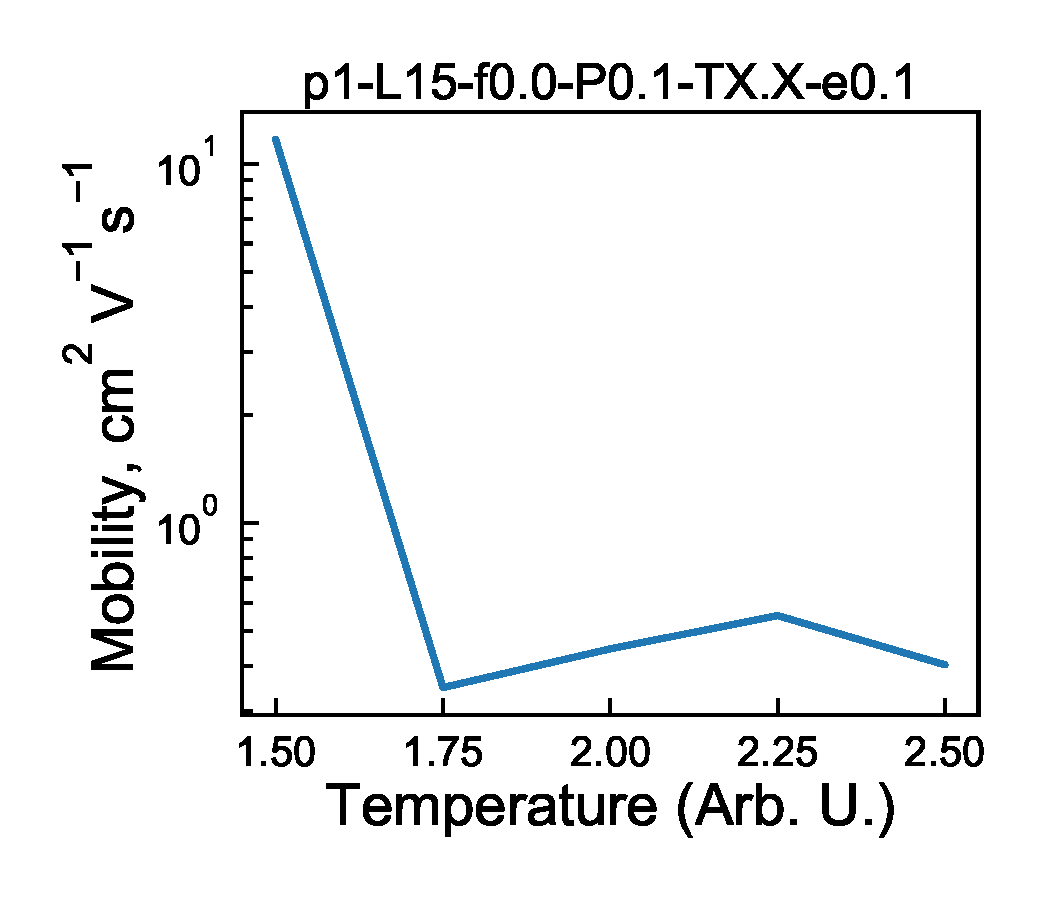
\includegraphics[width=0.5\textwidth]{Figures/origP3HTMob.pdf}&
        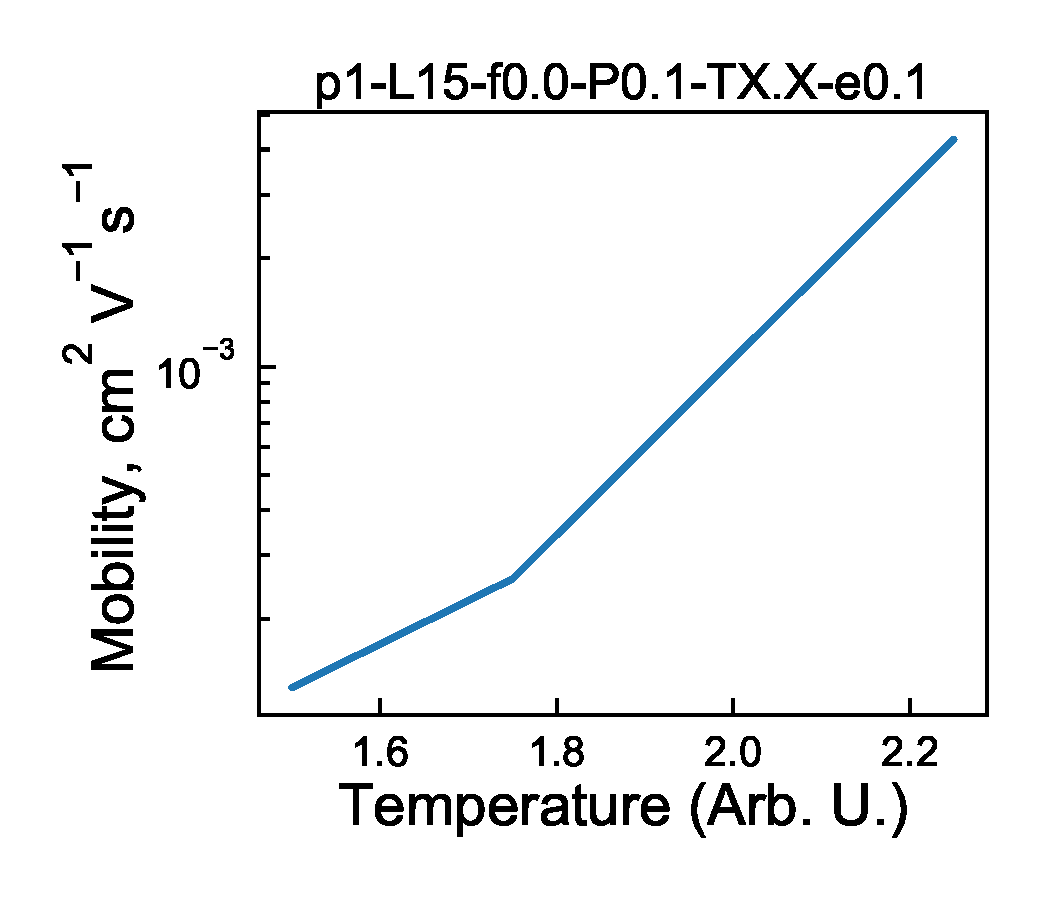
\includegraphics[width=0.5\textwidth]{Figures/newP3HTMob.pdf}
    \end{tabular}
    \caption{The evolution of the mobility of the p1-L15-f0.0-P0.1-TX.X-e0.5 systems.
        Left: Original P3HT mobility curve.
        Right: P3HT mobility curve when the Gaussian mapping is not performed.
}
	\label{fig:mob}
\end{figure}

\clearpage



\begin{figure}[h]\centering
	\includegraphics[width=0.85\textwidth]{Figures/P3HT-T1.5-noMap.png}
    \caption{   1) Chromophore connectivity network, 
                2) Location of `stacks', 
                3) Distribution of connected chromophore separations (defines stacks),
                4) Density of states of Frontier molecular orbital (delta Eij),
                5) KMC Carrier termination locations (defines anisotropy),
                6) Histogram of molecular transfer integrals,
                7) Histogram of stack transfer integrals,
                8) Histogram of molecular hopping rates,
                9) Histogram of stack hopping rates,
                10) Linear MSD plot,
                11) Semi-log-x MSD plot,
                12) Logarithmic MSD plot.}
	\label{fig:T1.5}
\end{figure}


\begin{figure}[h]\centering
	\includegraphics[width=0.85\textwidth]{Figures/P3HT-T1.75-noMap.png}
    \caption{   1) Chromophore connectivity network, 
                2) Location of `stacks', 
                3) Distribution of connected chromophore separations (defines stacks),
                4) Density of states of Frontier molecular orbital (delta Eij),
                5) KMC Carrier termination locations (defines anisotropy),
                6) Histogram of molecular transfer integrals,
                7) Histogram of stack transfer integrals,
                8) Histogram of molecular hopping rates,
                9) Histogram of stack hopping rates,
                10) Linear MSD plot,
                11) Semi-log-x MSD plot,
                12) Logarithmic MSD plot.}
	\label{fig:T1.75}
\end{figure}



\begin{figure}[h]\centering
	\includegraphics[width=0.85\textwidth]{Figures/P3HT-T2.25-noMap.png}
    \caption{   1) Chromophore connectivity network, 
                2) Location of `stacks', 
                3) Distribution of connected chromophore separations (defines stacks),
                4) Density of states of Frontier molecular orbital (delta Eij),
                5) KMC Carrier termination locations (defines anisotropy),
                6) Histogram of molecular transfer integrals,
                7) Histogram of stack transfer integrals,
                8) Histogram of molecular hopping rates,
                9) Histogram of stack hopping rates,
                10) Linear MSD plot,
                11) Semi-log-x MSD plot,
                12) Logarithmic MSD plot.}
	\label{fig:T2.25}
\end{figure}


\newpage

\section{Discussion}

As expected, a system with a broader density of states will exhibit a lower mobility than one with a less-broad DoS.
What is not expected is that it seems that the ordered morphology $T = 1.5$ has a broader density of states than the disordered $T = 1.75$ and $T = 2.25$ systems.
As such, the mobility trend is reversed with the ordered system exhibiting a mobility half that of the lowest-temperature disordered system and an order of magnitude lower than the $T = 2.25$ system.
I will wait for the results from the $T = 2.0$ and $T = 2.5$ systems to come back before I dig any further here.



%
%
%\begin{figure}[h!]\centering
%	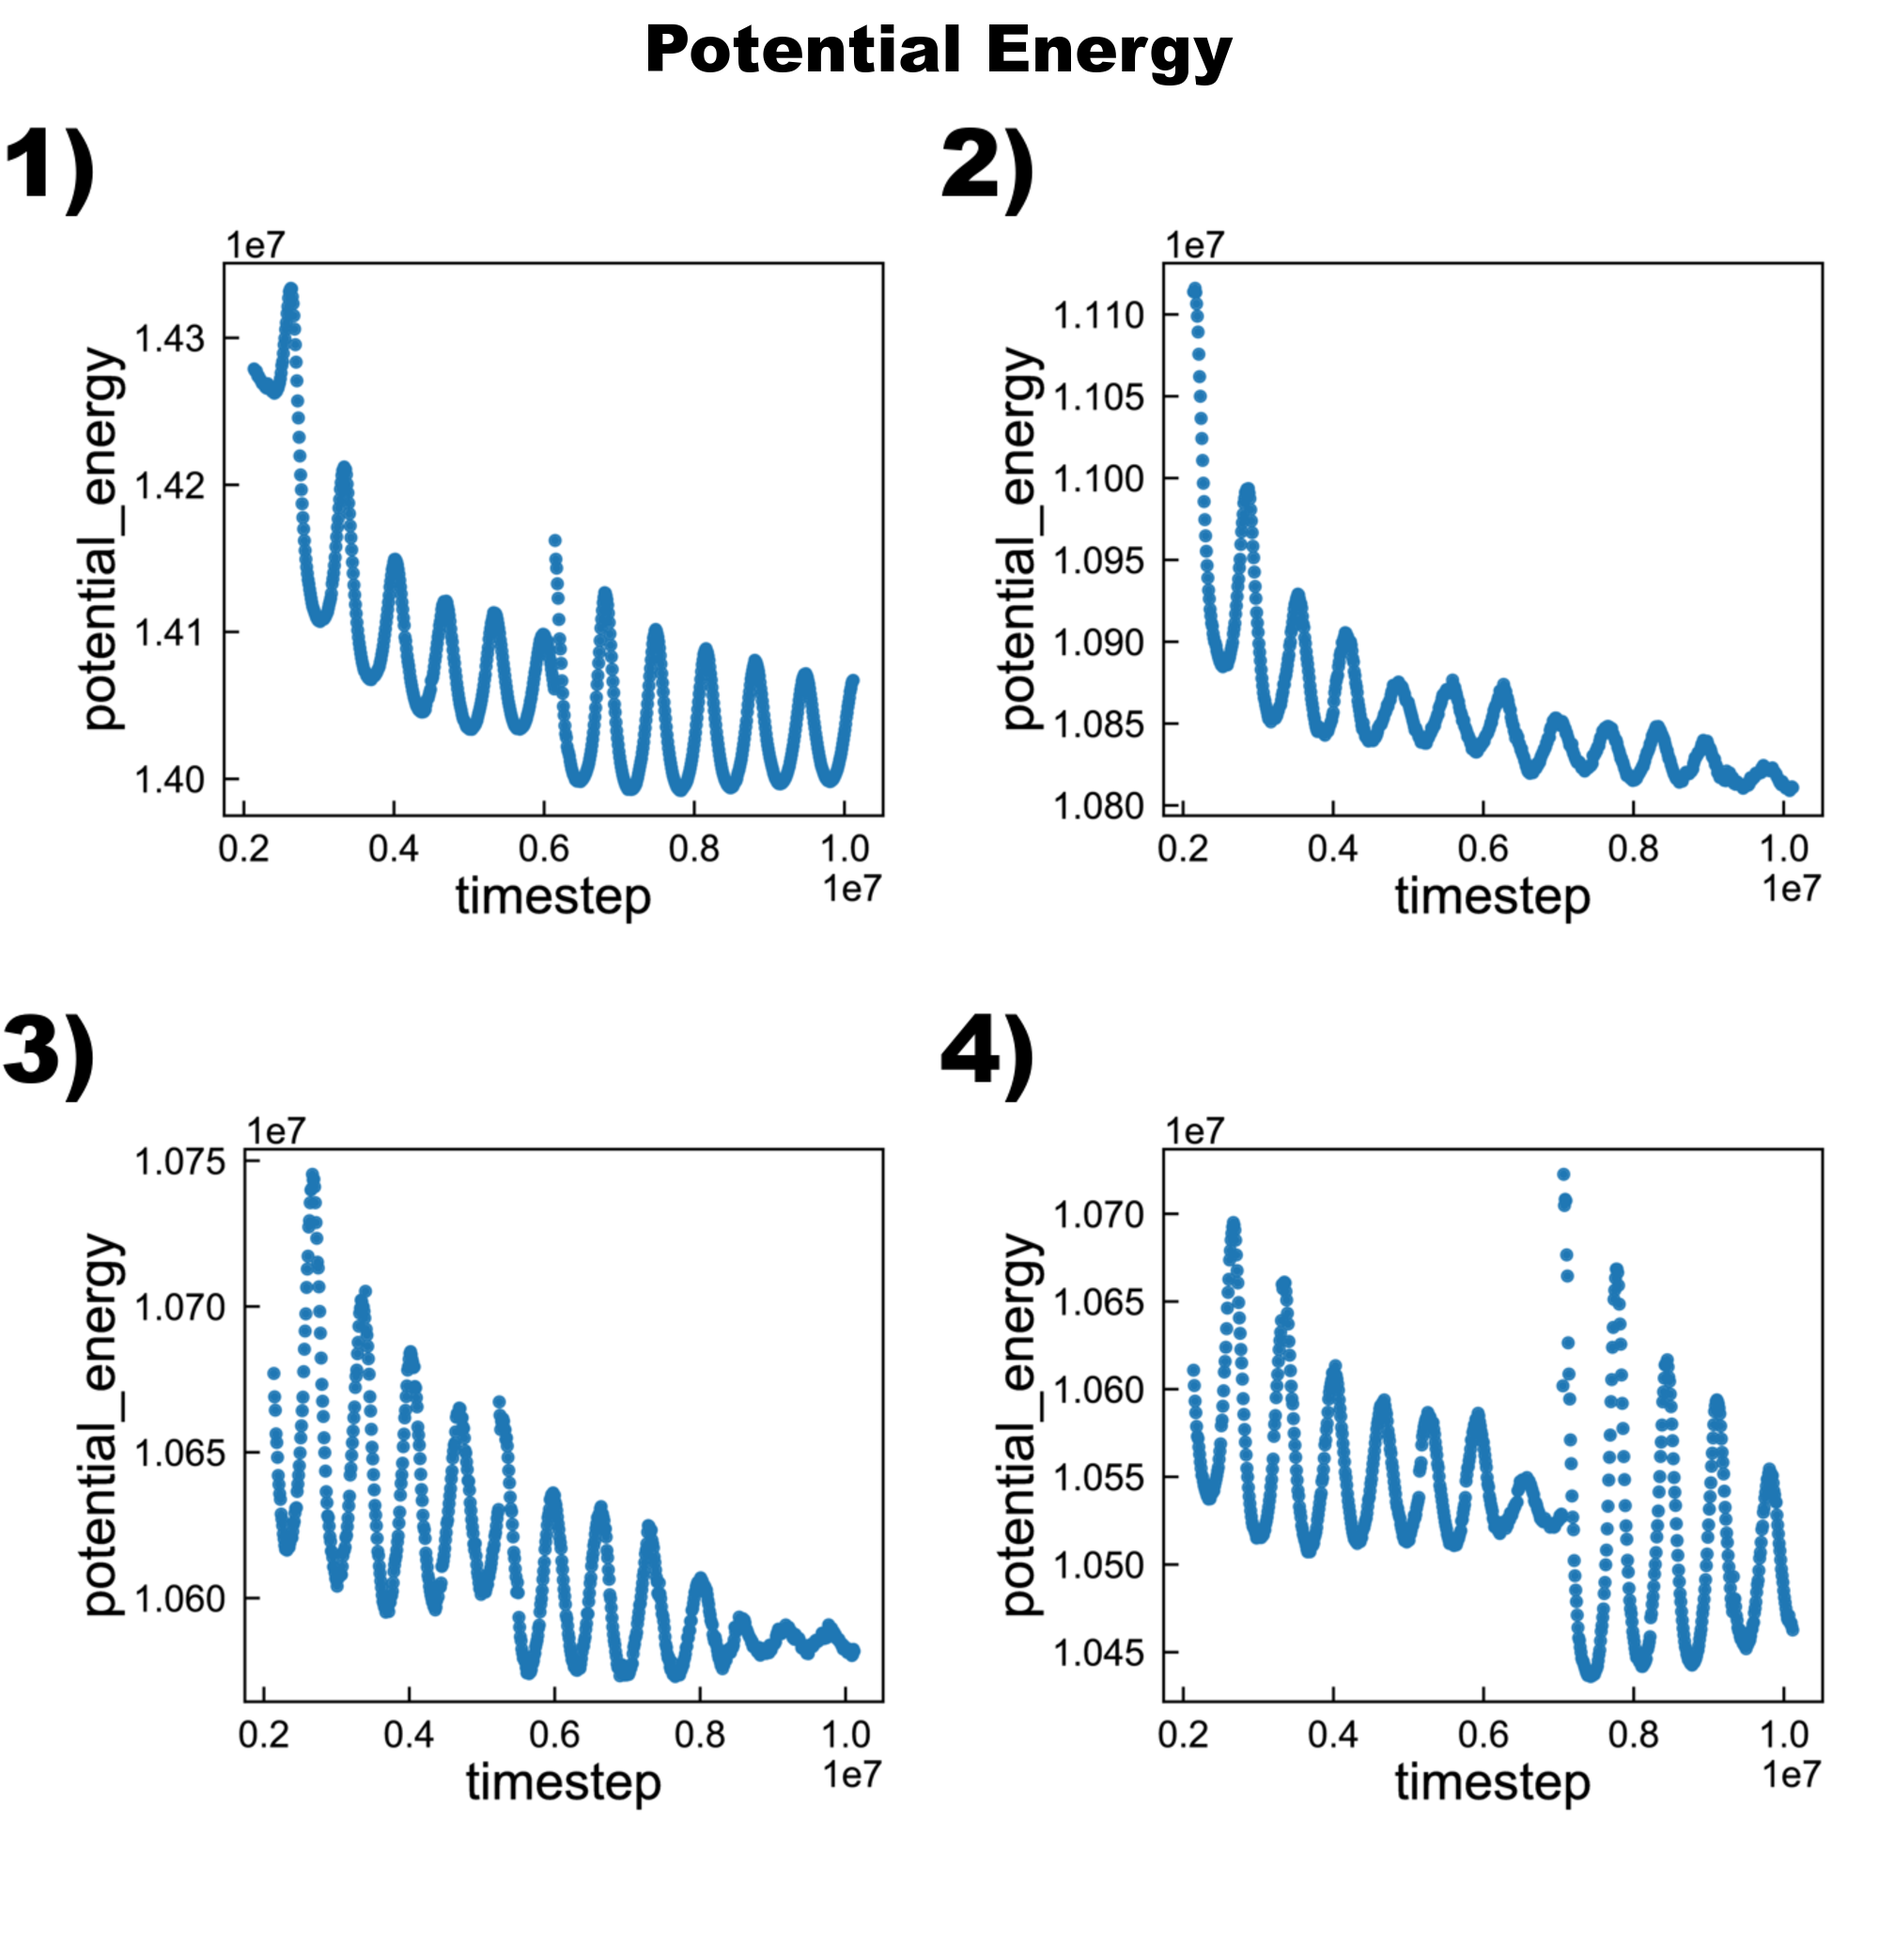
\includegraphics[width=\textwidth]{Figures/Potential_Energy.png}
%    \caption{The evolution of the total potential energy of the p1-L15-f0.0-P0.1-TX.X-e0.5 systems.
%        a) $T = 1.5$, b) $T = 1.75$, c) $T = 2.0$, d) $T = 2.25$.
%    The potential energy was dumped 1000 times for each phase, and only the final 800 energy values recorded are shown here.
%    The final phase ran 1E7 timesteps of 1E-5s each.
%}
%	\label{fig:PE}
%\end{figure}
%
%
%\textcolor{red}{Not going to report the mobilities until we are happy with the equilibration first.}


\bibliography{refs}
\bibliographystyle{unsrt}


\end{document}
